\chapter{Evaluation}

\section{Multimodal-MNIST}
We first look at applying the anomaly detection pipeline to Multimodal MNIST (MM-MNIST), proposed in \cite{ModDrop}. This dataset consists of the classic MNIST dataset, with each image split into quarters, giving four $14\times 14 \times 1$ pixel modalities. We implement a convolutional neural network with a separate head for each modality, and a tail which combines the head outputs and completes the classification [Table \ref{table:mm-mnist}].

\begin{table}[ht]
    \caption{MM-MNIST CNN classifier architecture}
    \centering
    \begin{tabular}{c c}
    \\
    \hline\hline
    \textbf{Layer} & \textbf{Kernel size/units} \\ [0.5ex]
    \hline
    \multicolumn{2}{c}{\textbf{Per-modality heads}} \\
    \hline
    Input & $14\times 14\times 1$ \\
    Dropout & $p=0.2$ \\
    Conv1 & $32\times 5 \times 5$ \\
    Conv2 & $32\times 3 \times 3$ \\
    MaxPool & $2\times 2$\\
    \hline
    \multicolumn{2}{c}{\textbf{Cross modality tail}} \\
    \hline 
    ModDrop & $p=0.1$ \\
    Conv3 & $64 \times 5 \times 5$ \\
    Conv4 & $64 \times 3 \times 3$ \\
    MaxPool & $2 \times 2$ \\
    Fully Connected & $10$ \\
    Log SoftMax & $10$ \\ [1ex] 
    \hline
    \end{tabular}
    \label{table:mm-mnist}
\end{table}
    
ModDrop \cite{ModDrop} is used before the tail to improve robustness to missing modalities as we intend to remove corrupt modalities at this stage. The classifier achieves 97.8\% accuracy on the test set.\\

We use the full GMM method above to generate a baseline for accuracy on corrupted data (Figure \ref{fig:baseline}). Repeated experiments across signal to noise ratio with 0, 1, or 2 corrupted modalities are carried out, and we measure accuracy on both the corrupted data, and the data with corrupted modalities zeroed out.

\begin{figure}[H]
    \centering\captionsetup{width=.8\linewidth}
    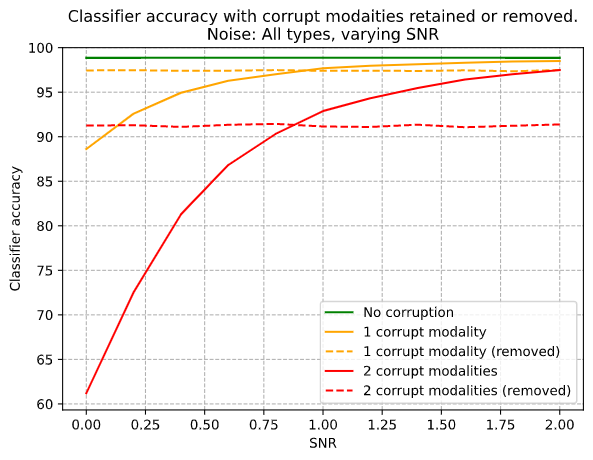
\includegraphics[width=.6\textwidth]{images/classifier_baseline.png}
    \caption{Baseline accuracy for corrupt and subsequently cleaned data with 0, 1 or 2 corrupted modalities. The MM-MNIST classifier appears robust to the noise used above a SNR of around 0.3 with 1 or 2 corrupt modalities. Beyond this threshold accuracy is greater if we don't attempt to clean the data.}
    \label{fig:baseline}
\end{figure}



We use the intermediate representations output by the head networks for anomaly detection. The outputs are flattened into 512 element vectors. The networks used in the first stage of DGCCA are fully connected, with layer sizes [512, 125, 64, 32]. These networks are trained on 50000 training samples, with the remaining 10000 held out for corruption detection training. Once the network heads are trained, a linear GCCA is trained on the resulting embeddings to produce transformations to the top $cca\_dim$ canonical variates.\\

The remaining 10000 elements of the training set are used for training the pairwise correlation thresholds. Correlations between DGCCA embeddings for each pair of modalities are measured on clean data and on data that has been corrupted with noise, picking the threshold as the intersection of the gaussians approximating the distributions of correlations. As we have 4 modalities, we learn 6 thresholds.\\

\todo{choice of params at this point?}

